\chapter{Methods}
\label{sec:methods}

\section{Robotic Platform}

The focus of this work is the application of tracking on humanoid robotic platforms where the manipulator is observed in a depth camera frame which is part of the robot's kinematic chain.

\subsection{Hardware}

The applied robot platform is the humanoid robot Valkyrie (\cref{fig:valkyrie}) which is developed by the NASA. It is \SI{1.8}{\meter} high and weights about \SI{125}{\kilo\gram}. In totally, it is actuated by 58 joints: leg ($2 \times 6$), arms ($2 \times 7$), hands ($2 \times 13$), neck (3) and torso (3). Hence, the kinematic chain from the observation frame to the hand frame consists of 10 actuated joints.

\begin{figure}
%\centering
\begin{minipage}{0.5\textwidth}
\centering
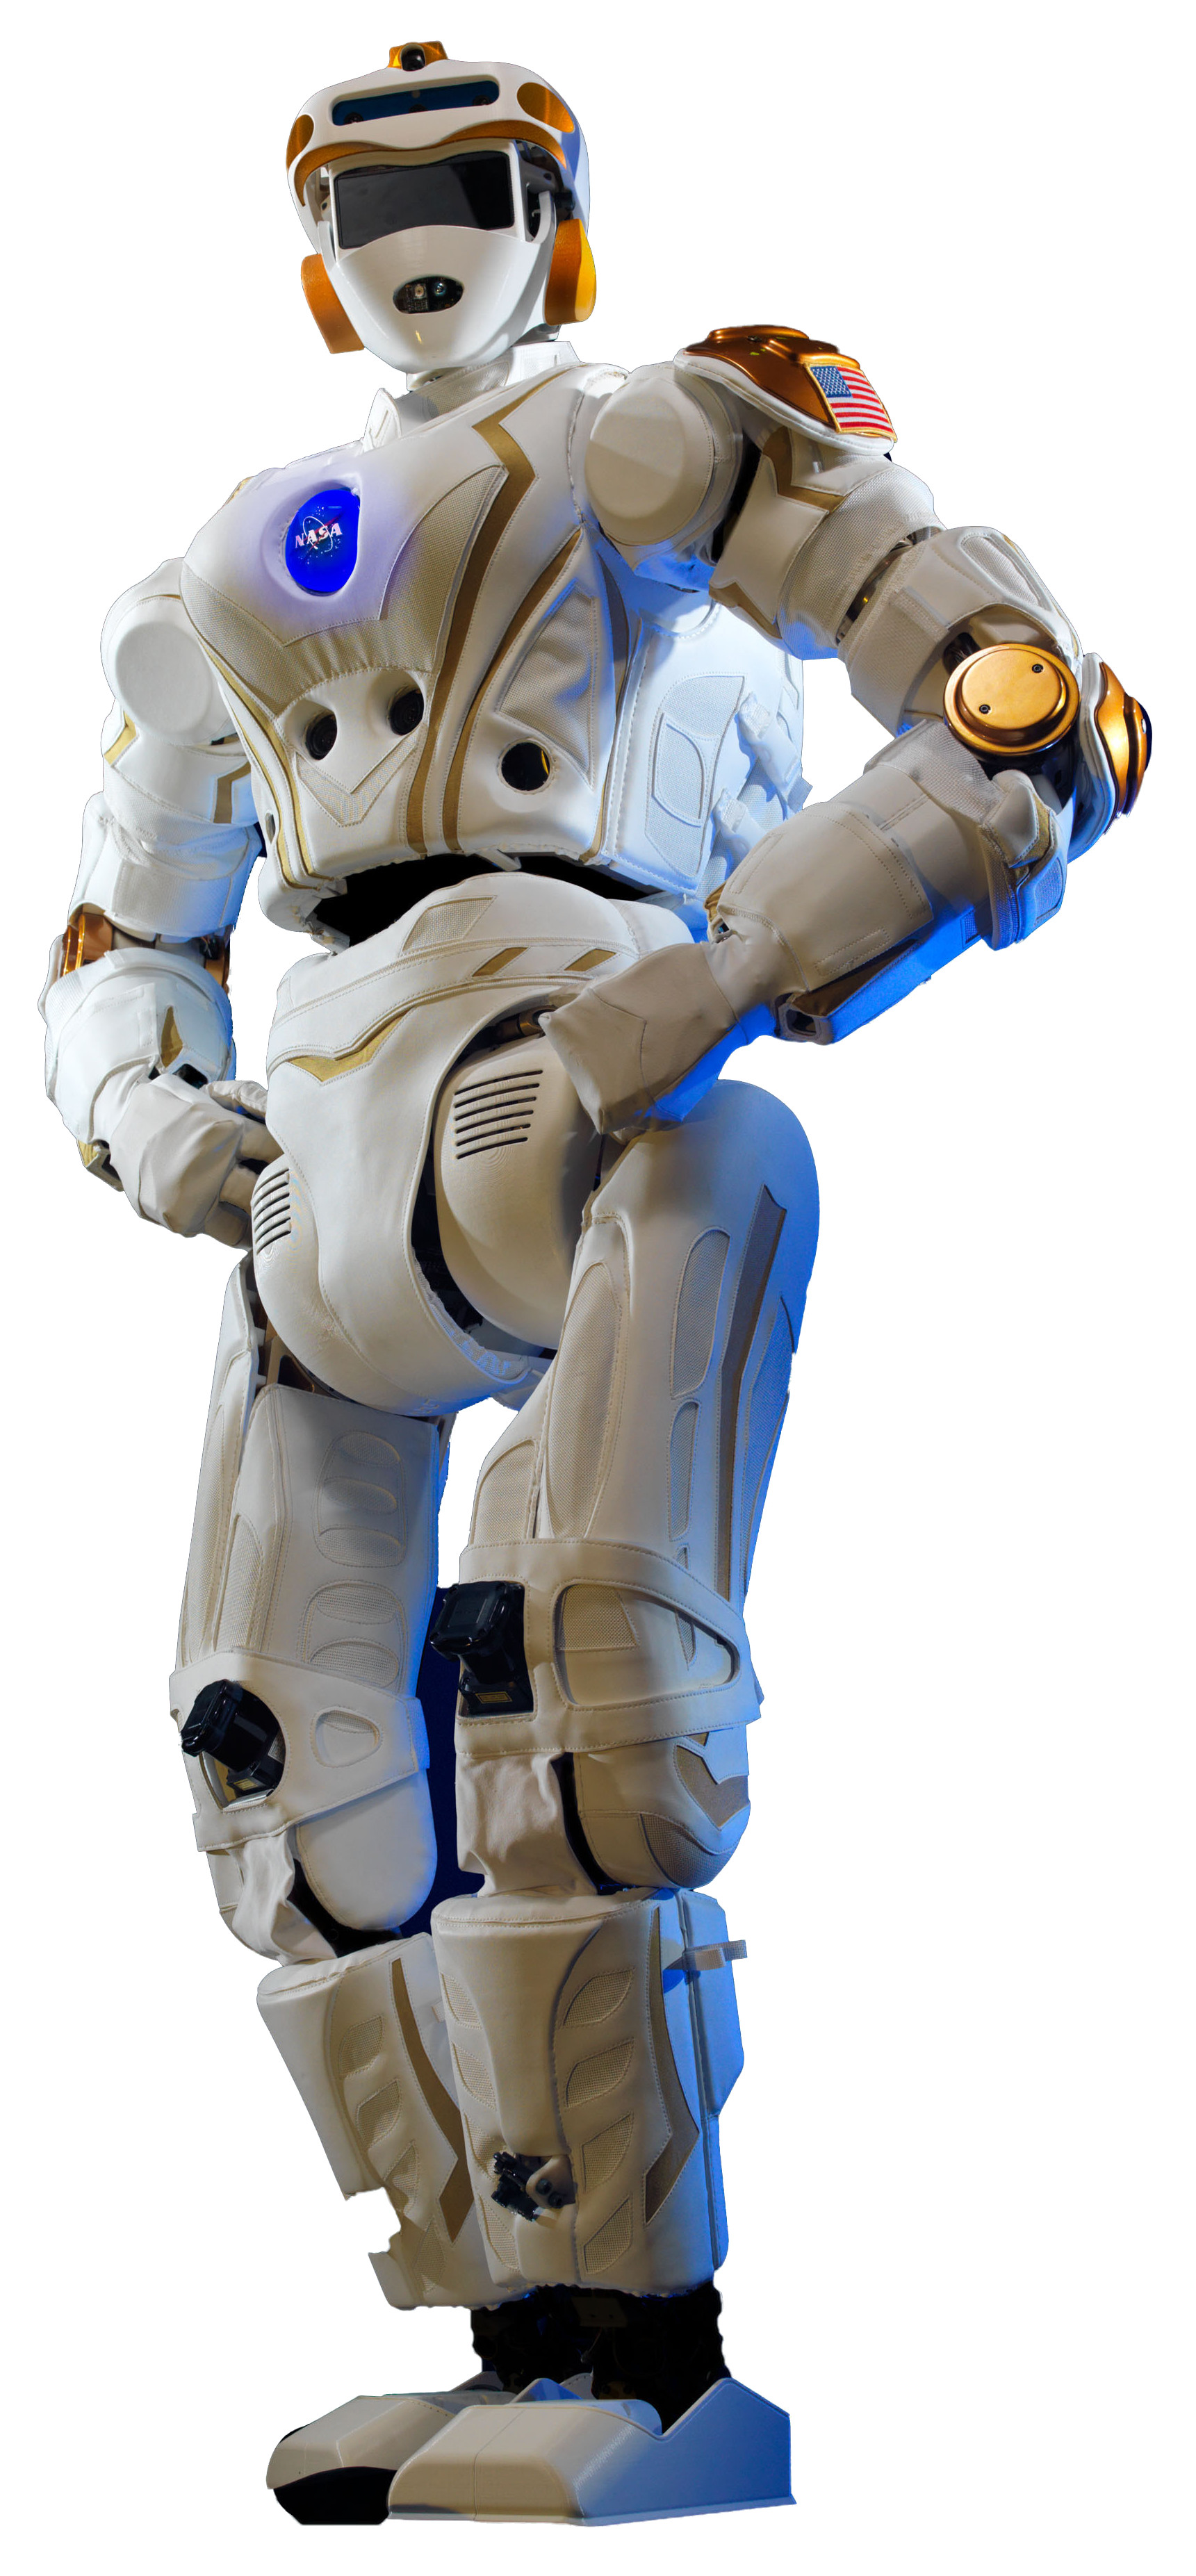
\includegraphics[width=0.6\textwidth]{images/valkyrie/Valkyrie.jpg}
\caption[Valkyrie]{Humanoid robot Valkyrie (Image credits: NASA)}
\label{fig:valkyrie}
\end{minipage}
%
\hspace{0.5cm}
%
\begin{minipage}{0.5\textwidth}
\centering
\subfloat[MultiSense SL]{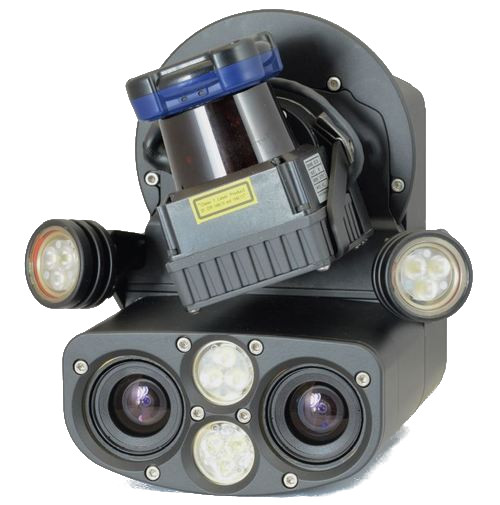
\includegraphics[width=0.8\textwidth]{images/valkyrie/MultiSense_SL.jpg} \label{fig:multisense}}

\subfloat[Asus Xtion PRO Live]{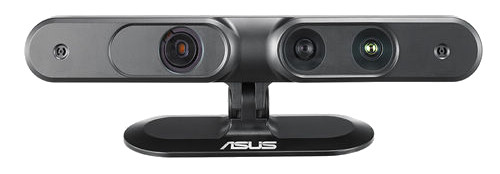
\includegraphics[width=0.8\textwidth]{images/valkyrie/xtion_pro_live.jpg} \label{fig:xtion_pro}}
\caption[Depth sensors]{Depth perception systems (Image credits: (a) Carnegie Robotics, (b) Asus)}
\label{fig:depth_sensors}
\end{minipage}
\end{figure}

The robot will use depth data as its main source of information for estimating the configuration of the manipulator and the object pose. The MultiSense SL stereo and LIDAR depth sensor (\cref{fig:multisense}), which is mounted inside the head of the robot, provides two sources of depth images: (1) stereo matching at \SI{15}{\hertz}, (2) rotating LIDAR which generates a full scan at \nicefrac{1}{6} \si{\hertz}. An optional structure from light sensor (\cref{fig:xtion_pro}), which can be mounted on top of the head, uses the known location of projected infrared (IR) dots to estimate the depth at these locations. The stereo cameras have their IR filter removed to enhance stereo matching by providing distinct keypoints from the IR pattern. The LIDAR data is not used for tracking because of its low update rate.
The key properties of both depth sensors are compared in \cref{tab:depth_sensor_comparison}. These properties are used for the back-projection to obtain the original 3D points.

\begin{table}
\captionsetup{width=0.7\textwidth}
\centering
\begin{tabular}{|c||c|c|}
\hline
 & \textit{MultiSense SL} & \textit{Asus Xtion PRO Live} \\
\hline
\hline
depth range & \SI{0.4}{\meter} - \SI{10}{\meter} & \SI{0.8}{\meter} - \SI{3.5}{\meter} \\
\hline
FOV & \SI{80}{\degree} $\times$ \SI{45}{\degree} & \SI{58}{\degree} $\times$ \SI{45}{\degree} \\
\hline
resolution & $1024 \times 1024$ & $640 \times 480$ \\
\hline
FPS & \SI{15}{\hertz} & \SI{30}{\hertz} \\
\hline
%f & \SI{6.5}{\milli\meter} & • \\
%\hline
$f_x$, $f_y$ & \SI{556.183}{pxl} & \SI{528.014}{pxl} \\
\hline
$c_x$, $c_y$ & \SI{512}{pxl} & (\SI{320}{pxl}, \SI{267}{pxl}) \\
\hline
b & \SI{0.07}{\meter} & \SI{0.075}{\meter} \\
\hline
\end{tabular}
\caption[Comparison of depth sensors]{Comparison of depth sensors. FOV: field of view, FPS: frames per second, $f$: focal length, $c$: image centre, $b$: baseline}
\label{tab:depth_sensor_comparison}
\end{table}


\subsection{Robot Model Representation}

Part of this thesis is the adaptation of DART's reference implementation to robot model representations stored in the URDF (Unified Robot Description Format) format. URDF defines at a minimum a tree structure that resembles the kinematic tree of a robot with its joints and links. It can additionally provide, among other things, information about joint limits and the geometric properties of the links. These geometric properties can be defined as primitive shapes like spheres, boxes or cylinders, or alternatively refer to complexer triangle meshes.

The URDF plugin for DART is designed that way, that all parts of the kinematic chain that are connected to a given root frame are tracked. This enables us to neglect robot parts that are not involved in manipulation. \Cref{fig:val_model_dart} shows such a model that is loaded from the \texttt{torso} frame upwards in the kinematic tree. Hence, it includes both arms, hands and the head with the sensors.
Having all these parts connected through a kinematic chain allows us to track both hands in a bimanual grasping task with respect to the camera frame without invalidating kinematic constraints, such as overrunning joint limits or disconnecting links.

\begin{figure}[h]
\centering
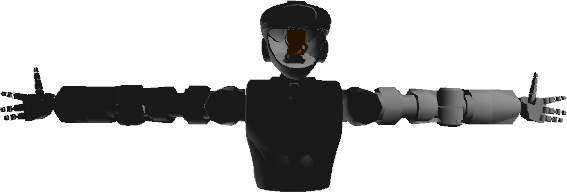
\includegraphics[width=\textwidth]{images/valkyrie/val_model_torso_dart.png}
\caption{Robot model loaded in DART}
\label{fig:val_model_dart}
\end{figure}


\section{Signed Distance Function}

The description of the signed distance function in this section is a reformulation based on the work by Schmidt et al. presented in \cite{Schmidt2015}.

The signed distance function (SDF) gives the shortest distance of a point in the observed point cloud to the robot model. It is signed in the sense that the distance is positive if the point lies outside the model, it is negative if the point is inside the model, and it is zero if the point lies exactly on the surface of the model. DART uses two kind of SDFs: the model SDF and the observation SDF.

The model SDF (\cref{fig:model_SDF}) gives the shortest distance of a point to a rigid model mesh. For articulated models, which consist of multiple such model meshes, a local model SDF is applied. This way, the complex computation of a global model SDF for each articulation can be broken down to the parallel computation of local SDFs per robot part. For each point in the point cloud, the distance to each robot part, respectively frame, is computed using the precomputed local SDFs. The point is then associated to the robot frame with the smallest absolute distance value.

In addition to considering observed data and the robot model, which is defined as \textit{positive information} in DART, the optimization is also using \textit{negative information}. If a point is observed in 3D, there cannot be anything in between this point and the camera centre. This free space constrain is visualised in \cref{fig:observation_SDF}. This observation SDF uses the distance transform on the observation and the estimated configuration of the model from the model SDF to constrain models to not be in free space.

\begin{figure}
\centering
\subfloat[Model SDF]{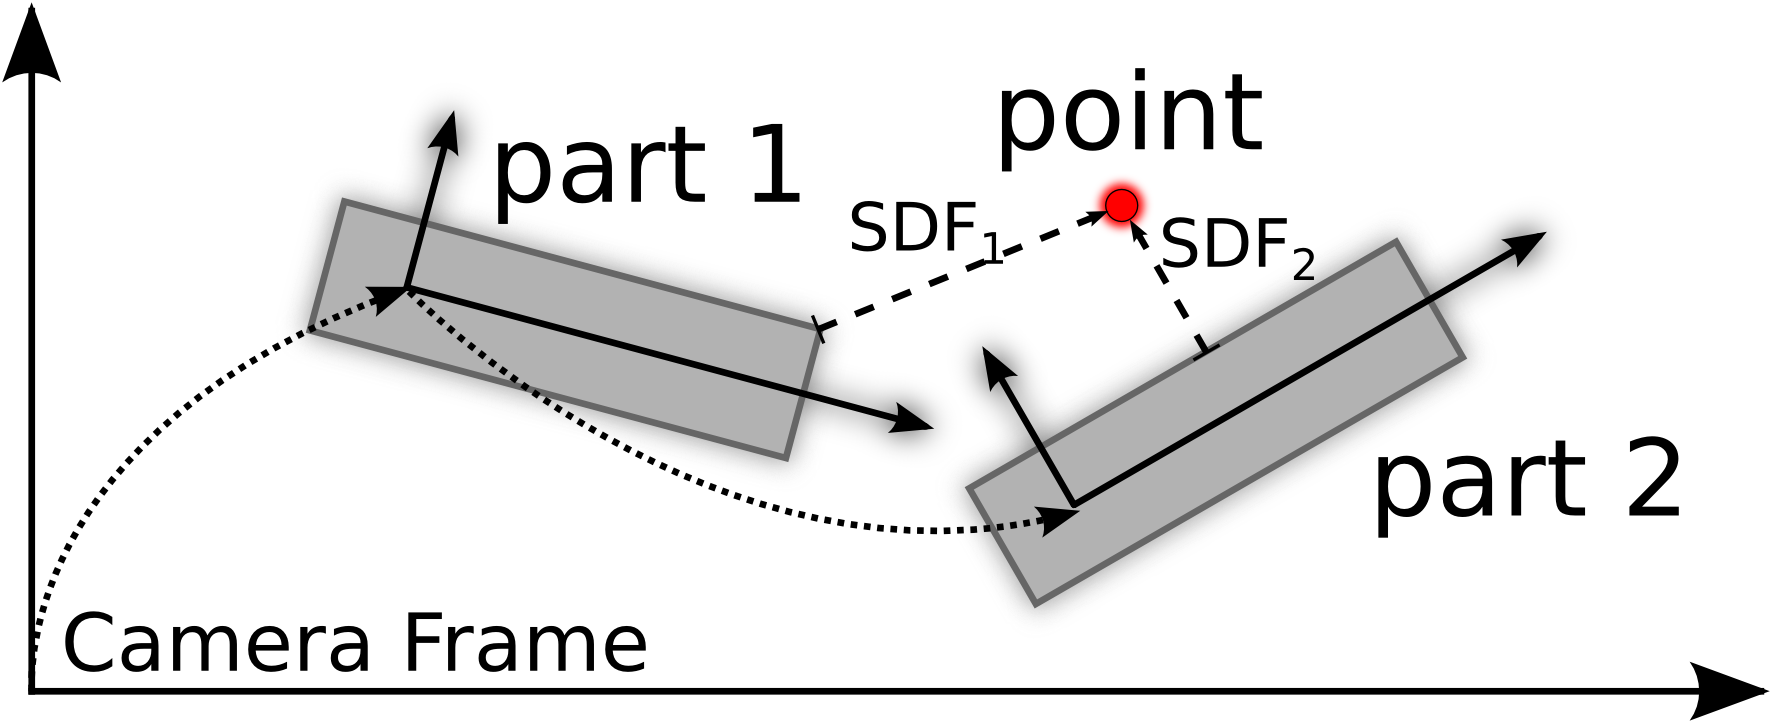
\includegraphics[width=0.5\textwidth]{images/sdf/local_sdf.png} \label{fig:model_SDF}}
\subfloat[Observation SDF]{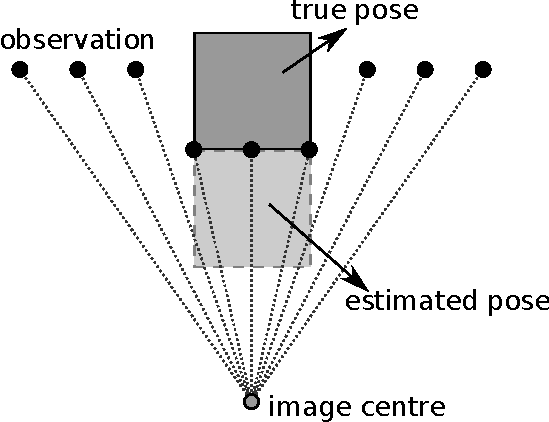
\includegraphics[width=0.3\textwidth]{images/sdf/sdf_obs.pdf} \label{fig:observation_SDF}}
\caption[Signed Distance Function]{Local model SDF and observation SDF (Inspired by \cite{Schmidt2015} figures 3 and 6). (a) the observed point is assigned to \emph{part 2}, (b) the estimated box (light gray) lies in between the observation and the image centre and thus invalidates the free space constrain.}
\end{figure}

\section{Gauss-Newton Algorithm}

The \textit{Gauss-Newton} algorithm is a method for finding the optimal set of parameters $\mathbf{p}$ that minimizes the sum of squares of non-linear vector-valued objective functions $e(\cdot)$
%
\begin{equation}
\hat{\mathbf{p}} = \arg\min_{p} \sum_{i=1}^N\left[ e_i(\mathbf{p})^2\right] .
\end{equation}

The Gauss-Newton algorithm is derived from the \textit{Newton} algorithm for finding roots and extremal points which itself is based on the Taylor series expansion. The Newton method for finding extremal points of the scalar objective function $f(\cdot)$ is an iterative procedure
%
\begin{equation}
x_{t+1} = x_t - \frac{f^{(1)}(x_t)}{f^{(2)}(x_t)}
\label{eqn:newton_minimum}
\end{equation}
%
starting at an initial state $x_0$ and using the first- and second-order derivatives ($f^{(1)}$, $f^{(2)}$) of the objective function to converge to a local minima.

For finding the minimum of a vector-valued function $e(\cdot)$ with respect to a parameter vector $\mathbf{p}$, the first- and second-order partial derivatives are used. In particular, the first- and second-order derivatives in \cref{eqn:newton_minimum} are replaced by the gradient $\nabla e(\mathbf{p})$ and the Hessian $\nabla^2 e(\mathbf{p})$ of the objective function $e$.
The partial derivatives of the vector-valued function $e(\cdot)$ with respect to the parameter vector $\mathbf{p}$ are aggregated in the \textit{Jacobian} matrix $J\in \mathbb{R}^{i \times j}$ with elements
%
\begin{align}
J_{i,j} &= \frac{\partial e_i(\mathbf{p})}{\partial p_j} .
\intertext{Hence,}
\nabla e(\mathbf{p}) &= J^\top e(\mathbf{p}) \label{eqn:gn_gradient}\\
H(e) = \nabla^2 e(\mathbf{p}) &= J^\top J +  \sum_{i=1} e_i(\mathbf{p}) \nabla^2 e_i(\mathbf{p}) \label{eqn:gn_hessian_full}.
\end{align}

For small $e$ close to an optimum, the Hessian $H(e)$ can be approximated by
\begin{equation}
H(e) \approx J^\top J \label{eqn:gn_hessian}
\end{equation}
%
neglecting the second-order derivatives. This approximation is used in the Gauss-Newton algorithm and the parameter update step then becomes
%
\begin{align}
\mathbf{p}_{t+1} &= \mathbf{p}_{t} - \Delta\mathbf{p} \\
&= \mathbf{p}_{t} - H(e)^{-1} \cdot \nabla e(\mathbf{p}) \\
&= \mathbf{p}_{t} - \left(J^\top J\right)^{-1} \cdot J^\top e(\mathbf{p}) \label{eqn:gn_param_update}.
\end{align}

The parameter update $\Delta\mathbf{p}$ is proportionally driven by the gradient of the objective function and scaled by the approximation of the Hessian. Because partial derivatives only consider the local change of the objective function, these gradient based approaches can only converge to local minimums.


\section{Prior Information}

Additional objective functions based on prior information can be integrated in the Gauss-Newton algorithm by blending their gradient and Hessian approximation with other objective functions. This is achieved by selecting an objective function and calculating its partial derivatives with respect to the parameter vector. These partial derivatives are used in the Jacobian as shown in \cref{eqn:gn_gradient,eqn:gn_hessian}.

The full parameter vector in DART consists of the 6D pose of the root frame and the $N$ joints positions:
\begin{equation}
\mathbf{p} = \begin{bmatrix}
x & y & z & \phi & \theta & \psi & | & q_1 & \cdots & q_N
\end{bmatrix}
\end{equation}
%
with $x$, $y$, $z$ for the translation, $\phi$, $\theta$, $\psi$ for the orientation in radiant Euler angles, and $q_1 \dots q_N$ the individual joint position values.


\subsection{Known Frame Pose}

As mentioned before, we know that the observation frame is part of the kinematic chain and rigidly connected to the head frame. Hence, observing this head frame is impossible.

For preventing movement of the head frame in between optimization iterations, the pose update in the parameter update vector $\Delta\mathbf{p}$ needs to be null. After the gradient and the Hessians of all other objective functions have been blended, the resulting gradient and Hessian is recomputed such that the pose update is removed from the parameter update vector.
From \cref{eqn:gn_param_update} the current parameter update is computed and its pose update is removed:
%
\begin{align}
\Delta\mathbf{p} &= \left(J^\top J\right)^{-1} \cdot J^\top e(\mathbf{p}) = \begin{bmatrix}
\mathbf{0} & | & q_1 & \cdots & q_N
\end{bmatrix} .
\intertext{This tampered parameter update vector is then used to compute a gradient that does not enforce a change in pose:}
J^\top e &= J^\top J \cdot \begin{bmatrix}
\mathbf{0} & | & q_1 & \cdots & q_N
\end{bmatrix} .
\end{align}

The final merged Hessian and the new gradient are the Gauss-Newton parameters that are used to compute the final parameter update.

\subsection{Reported Joint Positions}

We use the reported state of the robot in a way, that we can drag the estimated solution away from possibly distracting perceptions towards the state perceived through the joint encoders.
Two different kind of objective functions have been selected for this purpose which compute a weighted deviation of the estimated joint configuration $\mathbf{q}$ from reported joint configuration $\mathbf{r}$. The deviation is defined as the L2 norm $\left( \lVert \cdot \rVert_2 \right)$ of the difference vector $\mathbf{d} = \mathbf{r} - \mathbf{q}$.
For all objective functions, $r_i$ and $q_i$ denote the individual joint positions in their corresponding configuration vector.

\begin{enumerate}
\item Weighted L2 norm of the estimated joint position deviation:
\begin{align}
e_1 &= w \cdot \lVert \mathbf{r} - \mathbf{q} \rVert_2 = \lVert w \cdot \mathbf{r} - \mathbf{q} \rVert_2 \\
&= w \cdot \sqrt{\sum_{i=1}^N (r_i - q_i)^2} \label{eqn:objf_weightedL2}
\intertext{
with scalar weight $w>0$.
\item Sum of squares of individually weighted joints:
}
e_2 &= \lvert \mathbf{r} - \mathbf{q} \rvert^\top Q \lvert \mathbf{r} - \mathbf{q} \rvert \\
&= \sum_{i=1}^N \left[ (r_i-q_i) \cdot \sum_{j=1}^N (r_j-q_j) \cdot \omega_{i,j} \right] \label{eqn:objf_indiv_weighted}
\end{align}
with the weight matrix $Q\in\mathbf{R}^{N\times N}$ and its elements $\omega_{i,j}$. As a error metric, the weight matrix $Q$ must be \emph{positive-semidefinite}. That is, $\forall \mathbf{x}\in\mathbf{R}^n: x^\top Q x \geq 0$.
\end{enumerate}

Whereas the first objective function (\cref{eqn:objf_weightedL2}) uses a common scalar weight for all joint deviations, the second objective function (\cref{eqn:objf_indiv_weighted}) can penalize specific joint deviations and specific linear combinations of deviations. This enables us to enforce a reported state onto the estimated state for specific parts of the robot while keeping other parts free to be optimized by other objective functions.

The respective partial derivatives for the Jacobian are:
\begin{enumerate}
\item Weighted L2 norm of the estimated joint position deviation:
\begin{align}
J_{ji} &= \frac{\partial e_1}{\partial q_i} = -w \frac{r_i - q_i}{\lVert \mathbf{r} - \mathbf{q} \rVert}
\intertext{\item Sum of squares of individually weighted joints:}
J_{ji} &= \frac{\partial e_2}{\partial q_i} = - \left[ \sum_{j=1}^N d_jq_{i,j}\right] + \left[ \sum_{j=1 \neq i}^N d_jq_{j,i}\right]
\end{align}
\end{enumerate}


\section{Ground Truth Data Collection}

To evaluate the tracking performance and verify the effect of the joint position prior, reference measurements of the true state of the robot are required. The Vicon motion caption system is selected to externally track the pose of IR reflective markers rigidly attached to the robot.

\subsection{Setup}

To obtain the true transformation from the pelvis frame to the left hand palm frame, reflective markers are rigidly mounted with standoffs to the specific robot frames. The photograph in \cref{fig:vicon_marker} shows the highlighted location of the markers on the \texttt{pelvis} frame (green) and the \texttt{leftPalm} frame (red).

\begin{figure}[h]
\captionsetup{width=0.4\textwidth}
\centering
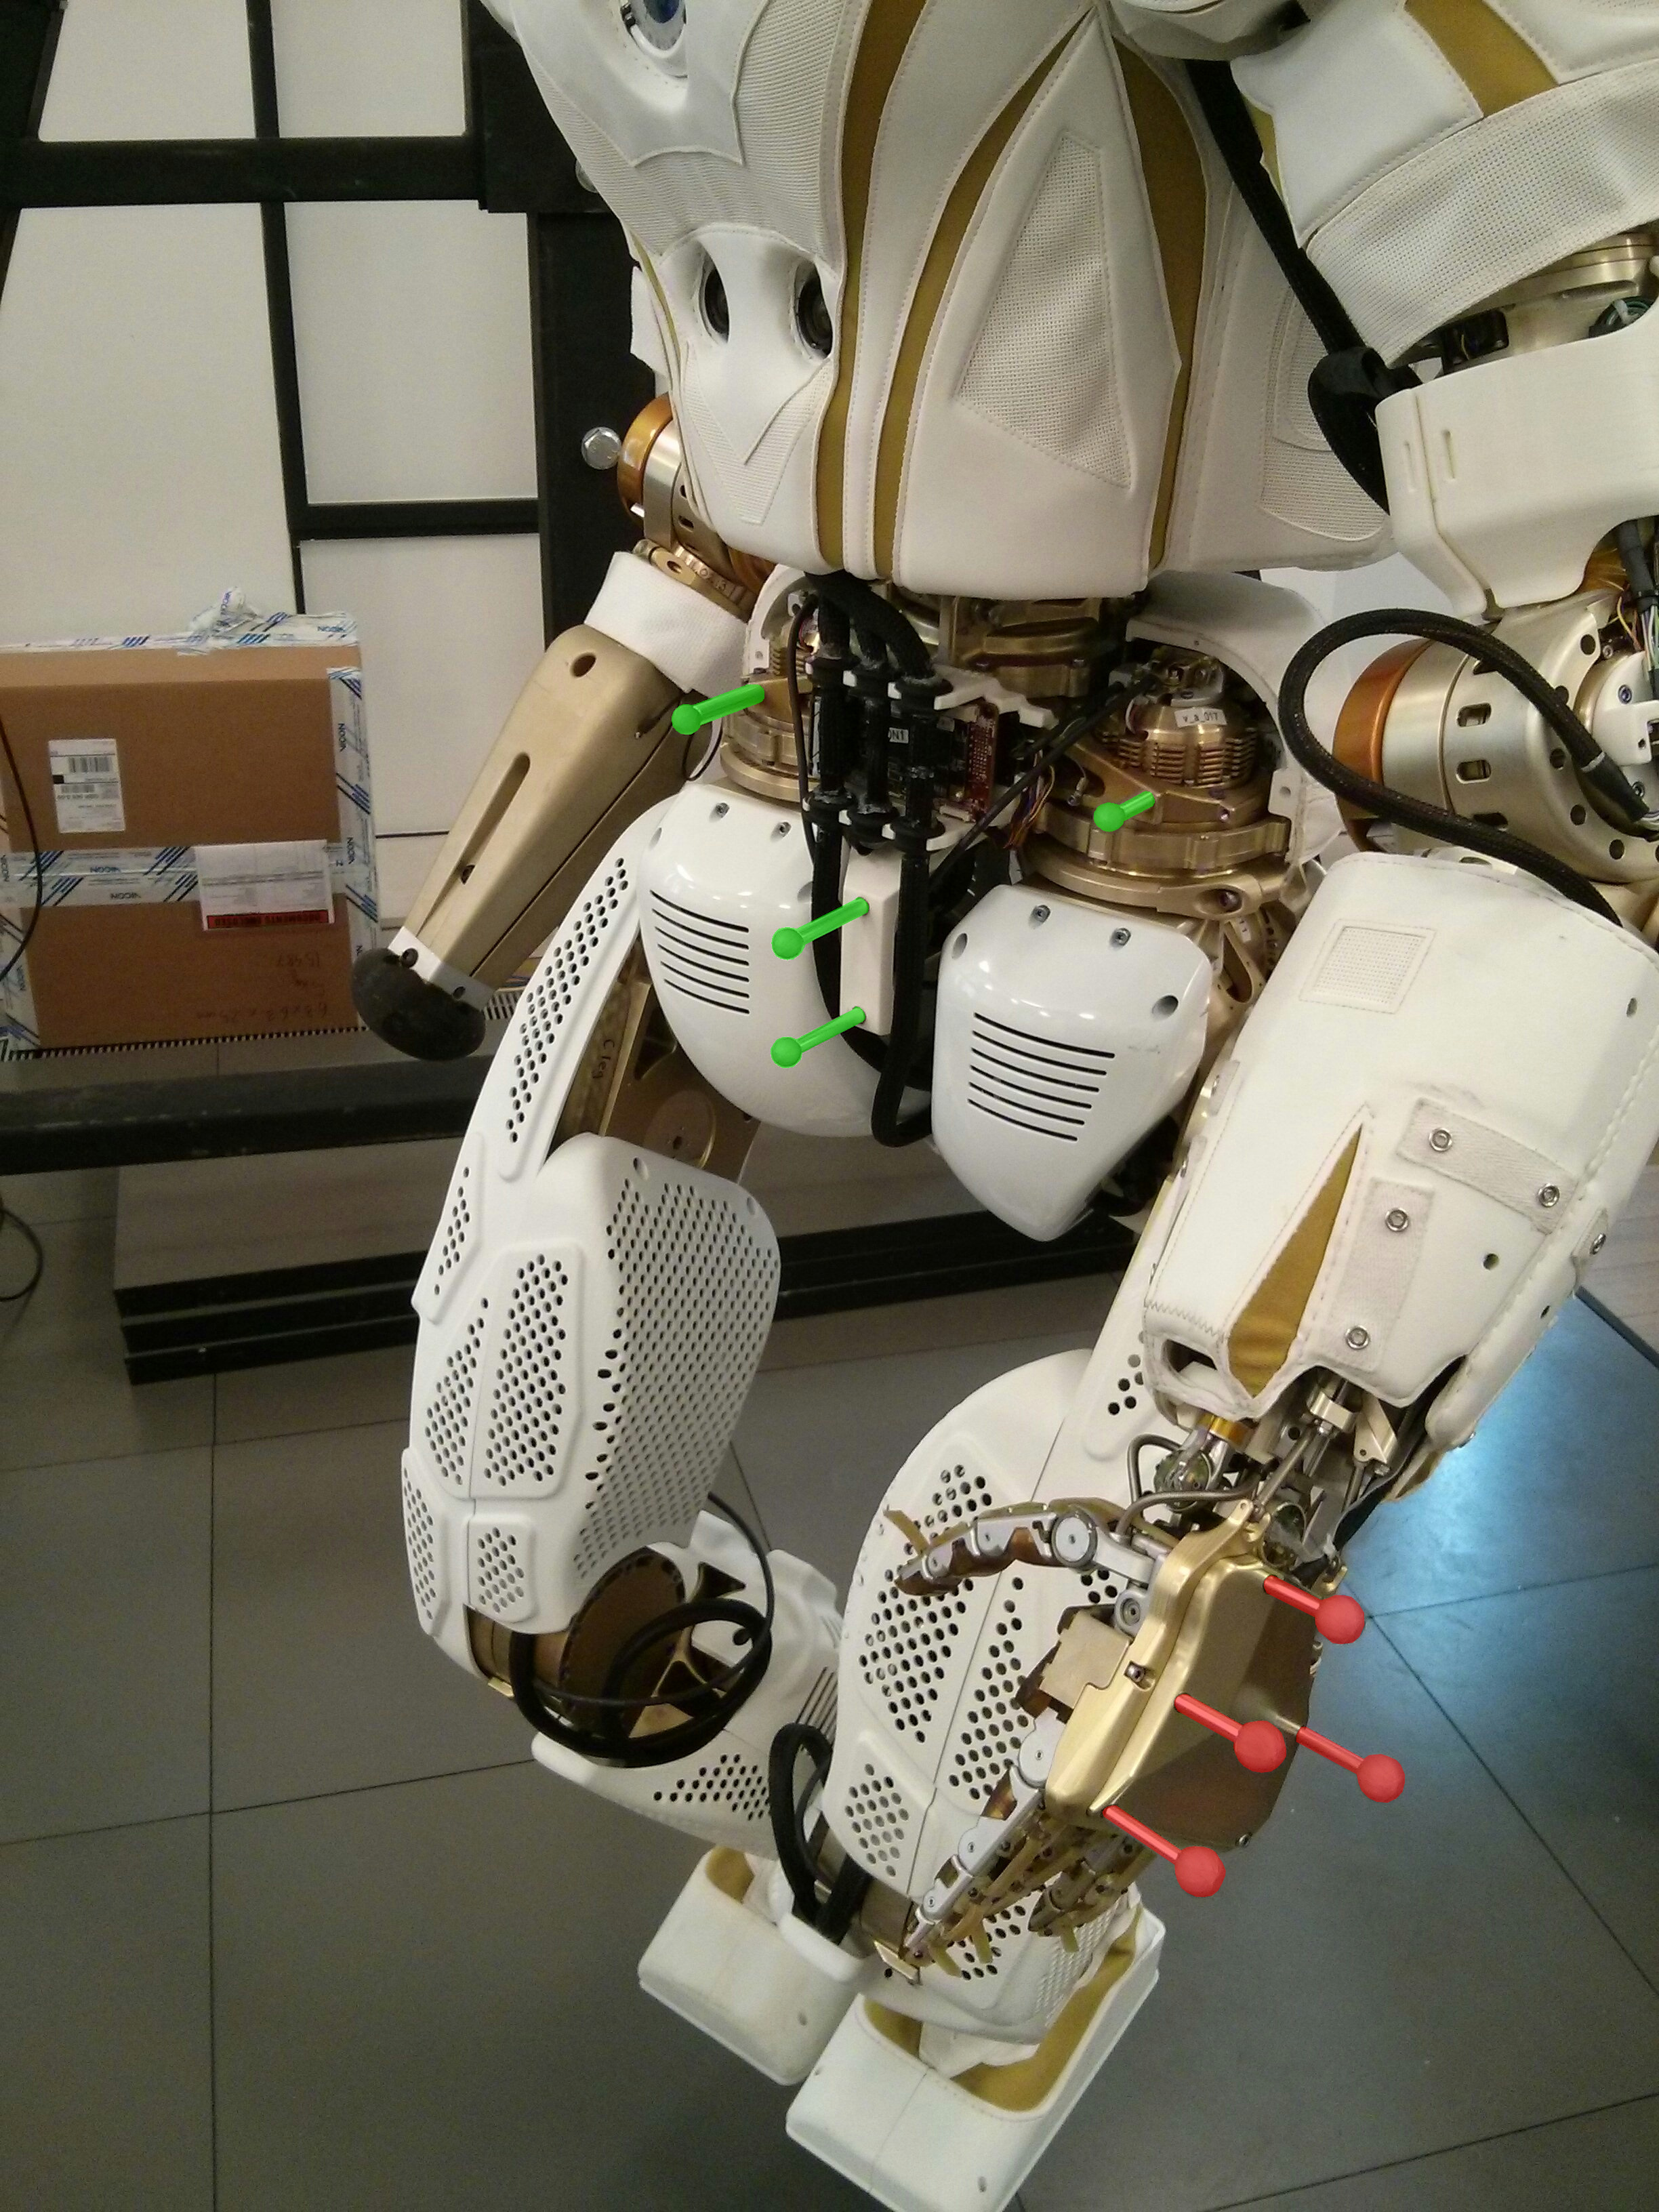
\includegraphics[width=0.4\textwidth]{images/vicon_pose/vicon_marker_col.jpg}
\caption[Location of Vicon marker]{Location of Vicon marker on pelvis (green) and left hand (red)}
\label{fig:vicon_marker}
\end{figure}


\subsection{Hand Pose}

Each group of markers has its own coordinate system with its origin in the centre.
The drawing in \cref{fig:transform_vicon_robot} visualizes the transformations between the Vicon world frame, the Vicon marker frames and the robot frames.
The transformations $T_{w \rightarrow vp}$ and $T_{w \rightarrow vh}$ are the reported poses of the Vicon marker in the world frame.
To obtain the transformation $T_{p \rightarrow h}$, which gives the hand pose in the pelvis frame, we need to find the rigid transformation between the Vicon marker and robot frame ($T_{m \rightarrow p}$ and $T_{m \rightarrow h}$).

\begin{figure}
\captionsetup{width=0.52\textwidth}
\centering
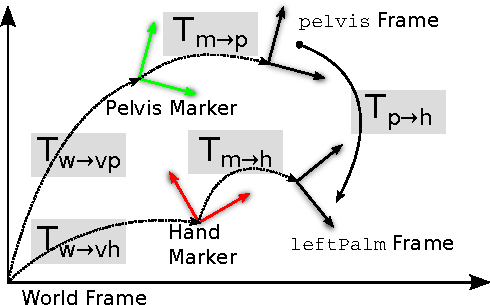
\includegraphics[width=0.5\textwidth]{images/vicon_pose/vicon_transforms.pdf}
\caption[Transformations of Vicon markers]{Transformations between Vicon markers (\textit{pelvis} - green, \textit{hand} - red) and robot frames}
\label{fig:transform_vicon_robot}
\end{figure}

The rigid transformation between marker and robot frames can be obtained by a least-squares optimization on corresponding points in both frames \cite{Umeyama1991}. Given corresponding points $m_i$ in marker frame and $x_i$ in the robot frame, the optimal projection of marker points from the marker frame into corresponding points in the robot frame becomes
\begin{equation}
T_{x \rightarrow m} = \arg\min_{R,t} \frac{1}{N} \sum_{i=1}^N \lVert x_i - \left( R \cdot m_i + t \right) \rVert_2
\label{eqn:least_squares_transformation_estimation}
\end{equation}
where $T_{x \rightarrow m}$ denotes the homogeneous transformation matrix containing the rotation matrix $R$ and the translation vector $t$. The points $x_i$ in the robot frame are here interchangeable for points $p_i$ in the \texttt{pelvis} frame and $h_i$ in the \texttt{leftPalm} frame. In particular, as result of this optimization we obtain $T_{p \rightarrow m}$ and $T_{h \rightarrow m}$.

%The Vicon system provides the pose of the marker frame in the world coordinate frame. That is the inverse of the transformations $T_{w \rightarrow vp}^{-1}$ and $T_{w \rightarrow vh}^{-1}$, e.g. the projection of the marker into the world frame.
The pose of the \texttt{pelvis} and \texttt{leftPalm} frame in the Vicon world frame can be expressed by the transformations
\begin{align}
T_{w \rightarrow p} &= T_{w \rightarrow vp} \cdot T_{m \rightarrow p} = T_{w \rightarrow vp} \cdot T_{p \rightarrow m}^{-1} \\
T_{w \rightarrow h} &= T_{w \rightarrow vh} \cdot T_{m \rightarrow h} = T_{w \rightarrow vh} \cdot T_{h \rightarrow m}^{-1} .
\end{align}

The transformations between these robot frames then finally becomes
\begin{align}
T_{w \rightarrow h} &= T_{w \rightarrow p} \cdot T_{p \rightarrow h} \\
T_{w \rightarrow vh} \cdot T_{h \rightarrow m}^{-1} &= T_{w \rightarrow vp} \cdot T_{p \rightarrow m}^{-1} \cdot T_{p \rightarrow h} \nonumber \\
T_{p \rightarrow h} &= \left( T_{w \rightarrow vp} \cdot T_{p \rightarrow m}^{-1} \right)^{-1} \cdot T_{w \rightarrow vh} \cdot T_{h \rightarrow m}^{-1} \label{eqn:hand_pose_from_vicon} .
\end{align}

Given the transformations of the Vicon markers ($T_{w \rightarrow vp}$ and $T_{w \rightarrow vh}$) at each time instance, and the rigid transformation between robot frames and their attached markers ($T_{p \rightarrow m}$ and $T_{h \rightarrow m}$) we can recover the true pose of the hand in the pelvis frame ($T_{p \rightarrow h}$) using \cref{eqn:hand_pose_from_vicon}.


\subsection{Joint Position Offset Calibration}

The availability of a true transformation within the robot kinematic chain enables us to compare the reported hand pose from forward kinematics with the true hand pose and further, calibrate the joints in the kinematic chain such that this deviation is minimized.

For minimizing the joint position deviation and obtaining correction offsets, the same optimization approach as described in \cite{Fallon2015} is applied. That is, given a correction function that maps a reported joint position value to its corrected value, $f_{corr}: q_{rep,i} \mapsto q_{corr,i}$, and a mapping from this joint space configuration to the 	task space pose of the manipulator using forward kinematics, $\phi: \mathbf{q} \mapsto \mathbf{p}$, with the pose $\mathbf{p} \in SE(3)$, the optimal correction parameters can be found by minimising
\begin{equation}
e = \frac{1}{N} \sum_{i=1}^N  \lVert \phi \left( f_{corr}(q_{rep,i}) \right) - \mathbf{p}_i \rVert_2
\end{equation}
for $N$ samples, respectively poses. The average error is selected over the summed error to have comparable costs between varying lengths of sample sequences.

Two correction functions $f_{corr}$ have been selected. The constant correction
\begin{align}
f_{corr}(q_{rep}) &= q_{offset} + q_{rep}
\label{eqn:const_offset}
\intertext{
assumes a constant offset that is independent from the reported joint position value itself. Here, only one parameter per calibrated joint has to be optimized. A linear correction function
}
f_{corr}(q_{rep}) &= q_{offset} + m_1 \cdot q_{rep}
\label{eqn:linear_offset}
\end{align}
assumes an additional relation to the reported joint position value itself. In this case twice as much parameters need to be optimised.

To prevent overfitting of the optimized correction parameters on the data set, the optimization result must be applied to a dedicated test set that has not been used for optimization. This is especially the case for more complex correction functions.
